\documentclass{standalone}

\usepackage[T1]{fontenc}
\usepackage[utf8]{inputenc}
\usepackage{eulervm}
\usepackage{amsmath}
\usepackage{bm}
\usepackage{tikz}
\usepackage{environ}
\usepackage{circuitikz}

\usetikzlibrary{fit}
\usetikzlibrary{patterns}
\usetikzlibrary{arrows}
\usetikzlibrary{positioning}

\usepackage{color}

\definecolor{Comment}{RGB}{97,161,176}

\definecolor{btfGreen}{RGB}{51,160,44}
\definecolor{btfRed}{RGB}{190,60,90}

\definecolor{bleuUni}{RGB}{0, 157, 224}
\definecolor{marronUni}{RGB}{68, 58, 49}
\definecolor{grayMarronUni}{RGB}{60, 60, 60}
\definecolor{grayBleuUni}{RGB}{118, 118, 118}

\definecolor{bluecite}{HTML}{009DE0}

\definecolor{Paired-2}{RGB}{166,206,227}
\definecolor{Paired-1}{RGB}{31,120,180}
\definecolor{Paired-4}{RGB}{178,223,138}
\definecolor{Paired-3}{RGB}{51,160,44}
\definecolor{Paired-6}{RGB}{251,154,153}
\definecolor{Paired-5}{RGB}{227,26,28}
\definecolor{Paired-8}{RGB}{253,191,111}
\definecolor{Paired-7}{RGB}{255,127,0}
\definecolor{Paired-10}{RGB}{202,178,214}
\definecolor{Paired-9}{RGB}{106,61,154}
\definecolor{Paired-12}{RGB}{255,255,153}
\definecolor{Paired-11}{RGB}{177,89,40}
\definecolor{Accent-1}{RGB}{127,201,127}
\definecolor{Accent-2}{RGB}{190,174,212}
\definecolor{Accent-3}{RGB}{253,192,134}
\definecolor{Accent-4}{RGB}{255,255,153}
\definecolor{Accent-5}{RGB}{56,108,176}
\definecolor{Accent-6}{RGB}{240,2,127}
\definecolor{Accent-7}{RGB}{191,91,23}
\definecolor{Accent-8}{RGB}{102,102,102}
\definecolor{Spectral-1}{RGB}{158,1,66}
\definecolor{Spectral-2}{RGB}{213,62,79}
\definecolor{Spectral-3}{RGB}{244,109,67}
\definecolor{Spectral-4}{RGB}{253,174,97}
\definecolor{Spectral-5}{RGB}{254,224,139}
\definecolor{Spectral-6}{RGB}{255,255,191}
\definecolor{Spectral-7}{RGB}{230,245,152}
\definecolor{Spectral-8}{RGB}{171,221,164}
\definecolor{Spectral-9}{RGB}{102,194,165}
\definecolor{Spectral-10}{RGB}{50,136,189}
\definecolor{Spectral-11}{RGB}{94,79,162}
\definecolor{Set1-1}{RGB}{228,26,28}
\definecolor{Set1-2}{RGB}{55,126,184}
\definecolor{Set1-3}{RGB}{77,175,74}
\definecolor{Set1-4}{RGB}{152,78,163}
\definecolor{Set1-5}{RGB}{255,127,0}
\definecolor{Set1-6}{RGB}{255,255,51}
\definecolor{Set1-7}{RGB}{166,86,40}
\definecolor{Set1-8}{RGB}{247,129,191}
\definecolor{Set1-9}{RGB}{153,153,153}
\definecolor{Set2-1}{RGB}{102,194,165}
\definecolor{Set2-2}{RGB}{252,141,98}
\definecolor{Set2-3}{RGB}{141,160,203}
\definecolor{Set2-4}{RGB}{231,138,195}
\definecolor{Set2-5}{RGB}{166,216,84}
\definecolor{Set2-6}{RGB}{255,217,47}
\definecolor{Set2-7}{RGB}{229,196,148}
\definecolor{Set2-8}{RGB}{179,179,179}
\definecolor{Dark2-1}{RGB}{27,158,119}
\definecolor{Dark2-2}{RGB}{217,95,2}
\definecolor{Dark2-3}{RGB}{117,112,179}
\definecolor{Dark2-4}{RGB}{231,41,138}
\definecolor{Dark2-5}{RGB}{102,166,30}
\definecolor{Dark2-6}{RGB}{230,171,2}
\definecolor{Dark2-7}{RGB}{166,118,29}
\definecolor{Dark2-8}{RGB}{102,102,102}
\definecolor{Reds-1}{RGB}{255,245,240}
\definecolor{Reds-2}{RGB}{254,224,210}
\definecolor{Reds-3}{RGB}{252,187,161}
\definecolor{Reds-4}{RGB}{252,146,114}
\definecolor{Reds-5}{RGB}{251,106,74}
\definecolor{Reds-6}{RGB}{239,59,44}
\definecolor{Reds-7}{RGB}{203,24,29}
\definecolor{Reds-8}{RGB}{165,15,21}
\definecolor{Reds-9}{RGB}{103,0,13}
\definecolor{Greens-1}{RGB}{247,252,245}
\definecolor{Greens-2}{RGB}{229,245,224}
\definecolor{Greens-3}{RGB}{199,233,192}
\definecolor{Greens-4}{RGB}{161,217,155}
\definecolor{Greens-5}{RGB}{116,196,118}
\definecolor{Greens-6}{RGB}{65,171,93}
\definecolor{Greens-7}{RGB}{35,139,69}
\definecolor{Greens-8}{RGB}{0,109,44}
\definecolor{Greens-9}{RGB}{0,68,27}
\definecolor{Blues-1}{RGB}{247,251,255}
\definecolor{Blues-2}{RGB}{222,235,247}
\definecolor{Blues-3}{RGB}{198,219,239}
\definecolor{Blues-4}{RGB}{158,202,225}
\definecolor{Blues-5}{RGB}{107,174,214}
\definecolor{Blues-6}{RGB}{66,146,198}
\definecolor{Blues-7}{RGB}{33,113,181}
\definecolor{Blues-8}{RGB}{8,81,156}
\definecolor{Blues-9}{RGB}{8,48,107}


\begin{document}
  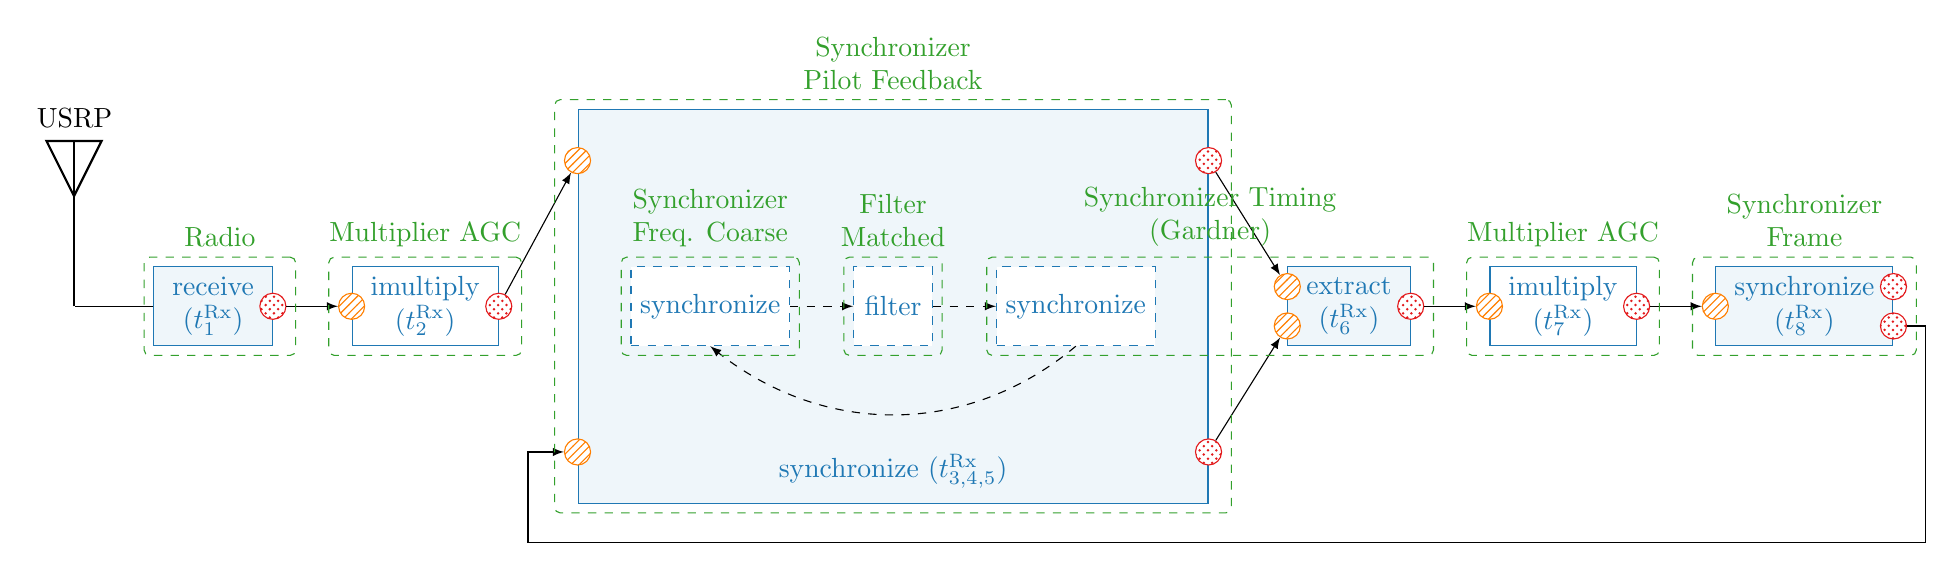
\begin{tikzpicture}%[scale=\tikzscale]
    \tikzset{ tsk/.style  ={draw=Paired-1, rounded corners=0pt, text=Paired-1, minimum height=1.0cm, minimum width=1cm} }
    \tikzset{ stsk/.style ={draw=Paired-1, rounded corners=0pt, text=Paired-1, minimum height=1.0cm, minimum width=1cm, fill=Paired-1!7} }
    \tikzset{ sutsk/.style={draw=Paired-1, rounded corners=0pt, text=Paired-1, minimum height=1.0cm, minimum width=1cm, preaction={fill=white}, dashed} }
    \tikzset{ ss/.style   ={draw=Paired-9, rounded corners=2pt, minimum height=1.5cm} }
    \tikzset{ seq/.style  ={draw=Paired-11, dashed, rounded corners=2pt} }
    \tikzset{ mdl/.style  ={draw=Paired-3,  dashed, rounded corners=2pt} }
    \tikzset{ pip/.style  ={draw=Dark2-8,  dotted, thick, rounded corners=2pt} }
    \tikzset{ sin/.style  ={draw=Paired-7, circle, minimum width=0.3cm, text=black, preaction={fill=white}, pattern=north east lines, pattern color=Paired-7} }
    \tikzset{ sout/.style ={draw=Paired-5, circle, minimum width=0.3cm, text=black, preaction={fill=white}, pattern=crosshatch dots, pattern color=Paired-5} }

    \node[stsk                     , align=center                                                                                                      ] (t1) at ( 0.0, 2.0) {~receive~~\\($t^{\text{Rx}}_1$)};
    \node[tsk ,  right=1.00cm of t1, align=center                                                                                                      ] (t2)                {~imultiply~~\\($t^{\text{Rx}}_2$)};
    \node[stsk,  right=1.00cm of t2, minimum width=8cm, minimum height=5cm, label={[Paired-1,yshift=0.75cm]below:synchronize ($t^{\text{Rx}}_{3,4,5}$)}] (t3)                {};
    \node[sutsk, at=(t3.center)                                                                                                                        ] (t3_2)              {filter};
    \node[sutsk, left =0.80cm of t3_2                                                                                                                  ] (t3_1)              {synchronize};
    \node[sutsk, right=0.80cm of t3_2                                                                                                                  ] (t3_3)              {synchronize};
    \node[stsk,  right=1.00cm of t3 , align=center                                                                                                     ] (t4)                {~extract~~\\($t^{\text{Rx}}_6$)};
    \node[tsk ,  right=1.00cm of t4 , align=center                                                                                                     ] (t5)                {~imultiply~~\\($t^{\text{Rx}}_7$)};
    \node[stsk,  right=1.00cm of t5 , align=center                                                                                                     ] (t6)                {~synchronize~~\\($t^{\text{Rx}}_8$)};

    \node[sout, at=(t1.east)                ] (t1_so)  {};
    \node[sin,  at=(t2.west)                ] (t2_si)  {};
    \node[sout, at=(t2.east)                ] (t2_so)  {};
    \node[sin,  at=(t3.west), yshift=+1.85cm] (t3_si1) {};
    \node[sin,  at=(t3.west), yshift=-1.85cm] (t3_si2) {};
    \node[sout, at=(t3.east), yshift=+1.85cm] (t3_so1) {};
    \node[sout, at=(t3.east), yshift=-1.85cm] (t3_so2) {};
    \node[sin,  at=(t4.west), yshift=+0.25cm] (t4_si1) {};
    \node[sin,  at=(t4.west), yshift=-0.25cm] (t4_si2) {};
    \node[sout, at=(t4.east)                ] (t4_so)  {};
    \node[sin,  at=(t5.west)                ] (t5_si)  {};
    \node[sout, at=(t5.east)                ] (t5_so)  {};
    \node[sin,  at=(t6.west)                ] (t6_si)  {};
    \node[sout, at=(t6.east), yshift=+0.25cm] (t6_so1) {};
    \node[sout, at=(t6.east), yshift=-0.25cm] (t6_so2) {};

    \draw[black, -] (t1.west)--++(0:-1.0cm) node[antenna, label={[above,yshift=+2.15cm]USRP}] {};
    \draw[->,>=latex        ] (t1_so)      --               (t2_si)       node [midway, above] {};
    \draw[->,>=latex        ] (t2_so)      --               (t3_si1)      node [midway, above] {};
    \draw[->,>=latex, dashed] (t3_1)       --               (t3_2)        node [midway, above] {};
    \draw[->,>=latex, dashed] (t3_2)       --               (t3_3)        node [midway, above] {};
    \draw[->,>=latex, dashed] (t3_3.south) to[bend left=40] (t3_1.south)  node [midway, above] {};
    \draw[->,>=latex        ] (t3_so1)     --               (t4_si1)      node [midway, above] {};
    \draw[->,>=latex        ] (t3_so2)     --               (t4_si2)      node [midway, above] {};
    \draw[->,>=latex        ] (t4_so)      --               (t5_si)       node [midway, above] {};
    \draw[->,>=latex        ] (t5_so)      --               (t6_si)       node [midway, above] {};

    \draw[->,>=latex] (t6_so2) -| (21.75,-1.0) -- (4.0,-1.0) |- (t3_si2)  node [midway, above] {};

    \node[mdl, label={[Paired-3, align=center]above:Radio},                          fit=(t1)           (t1_so)           ] (m1)  {};
    \node[mdl, label={[Paired-3, align=center]above:Multiplier AGC},                 fit=(t2)  (t2_si)  (t2_so)           ] (m2)  {};
    \node[mdl, label={[Paired-3, align=center]above:Synchronizer\\Pilot Feedback},   fit=(t3)  (t3_si1) (t3_si2)  (t3_so1)] (m3)  {};
    \node[mdl, label={[Paired-3, align=center]above:Synchronizer\\Freq. Coarse},     fit=(t3_1)                           ] (m4)  {};
    \node[mdl, label={[Paired-3, align=center]above:Filter\\Matched},                fit=(t3_2)                           ] (m5)  {};
    \node[mdl, label={[Paired-3, align=center]above:Synchronizer Timing\\(Gardner)}, fit=(t3_3) (t4) (t4_so)              ] (m6)  {};
    \node[mdl, label={[Paired-3, align=center]above:Multiplier AGC},                 fit=(t5)  (t5_si)  (t5_so)           ] (m7)  {};
    \node[mdl, label={[Paired-3, align=center]above:Synchronizer\\Frame},            fit=(t6)  (t6_si)  (t6_so1) (t6_so2) ] (m8)  {};
  \end{tikzpicture}
\end{document}